\section{Model hyperparameters}

Building the different models for the procedure illustrated in figure \ref{fig:model_training_concept} requires making several choices.
In this section, components and hyperparameters between which were chosen are introduced.

\subsection{Network types\label{sec:network_types}}

Three different \acrlong{cnn} architectures were tested for this project.
All three of these networks are based on the encoder-decoder principle where a contracting part of the network extracts \Gls{features} and an expanding layer sequence produces a segmentation mask.

\begin{description}
    \item[VGG16 network: ] This is a classic classification network, developed by K. Simonyan \& A. Zimmerman. 
    The used network is illustrated in figure \ref{fig:vgg16}. 
    Inspired by \cite{Laradji2021}, the network is adapted for segmentation (This segmentation architecture is called VGG16 FCN8) by omitting the flattening layer for image-level classification and replacing it with an upsampling path. In this upsampling path, the (expanded) pooling layers after conv3 and conv4 are added to the results with an element-wise summation.
    \item[U-Net network: ] The U-Net is a network specifically designed for segmentation tasks. As was already described in chapter \ref{sec:MachineVisionMedical} on page \pageref{sec:MachineVisionMedical}, 
    this network architecture was originally published in \cite{Ronneberger2015}.
    \item[RESNET50 network:] The \Gls{resnet} (Kaiming He et al.) is a classification architecture that can be made very deep (more than 150 layers).
    This depth is possible thanks to the skip connections. The network tested in this work implements the RESNET50 architecture, adapted with an FCN8 upsampling segmentation part.
    The RESNET50 architecture can be seen as a stack of \textit{residual units}. In figure \ref{fig:vgg16}, four such a residual block is illustrated.
    The number of feature maps is doubled every few residual units, while the height and width are halved. When this happens, the input cannot be added directly to the output of the residual unit.
    To solve this problem, the inputs are passed through a $1\times 1$ convolution layer with stride 2 and the correct number of output feature maps (the blue layer in figure \ref{fig:vgg16}).
\end{description}

\begin{SCfigure}[][htb]
    \centering
    \centering
    \begin{minipage}{.99\textwidth}
        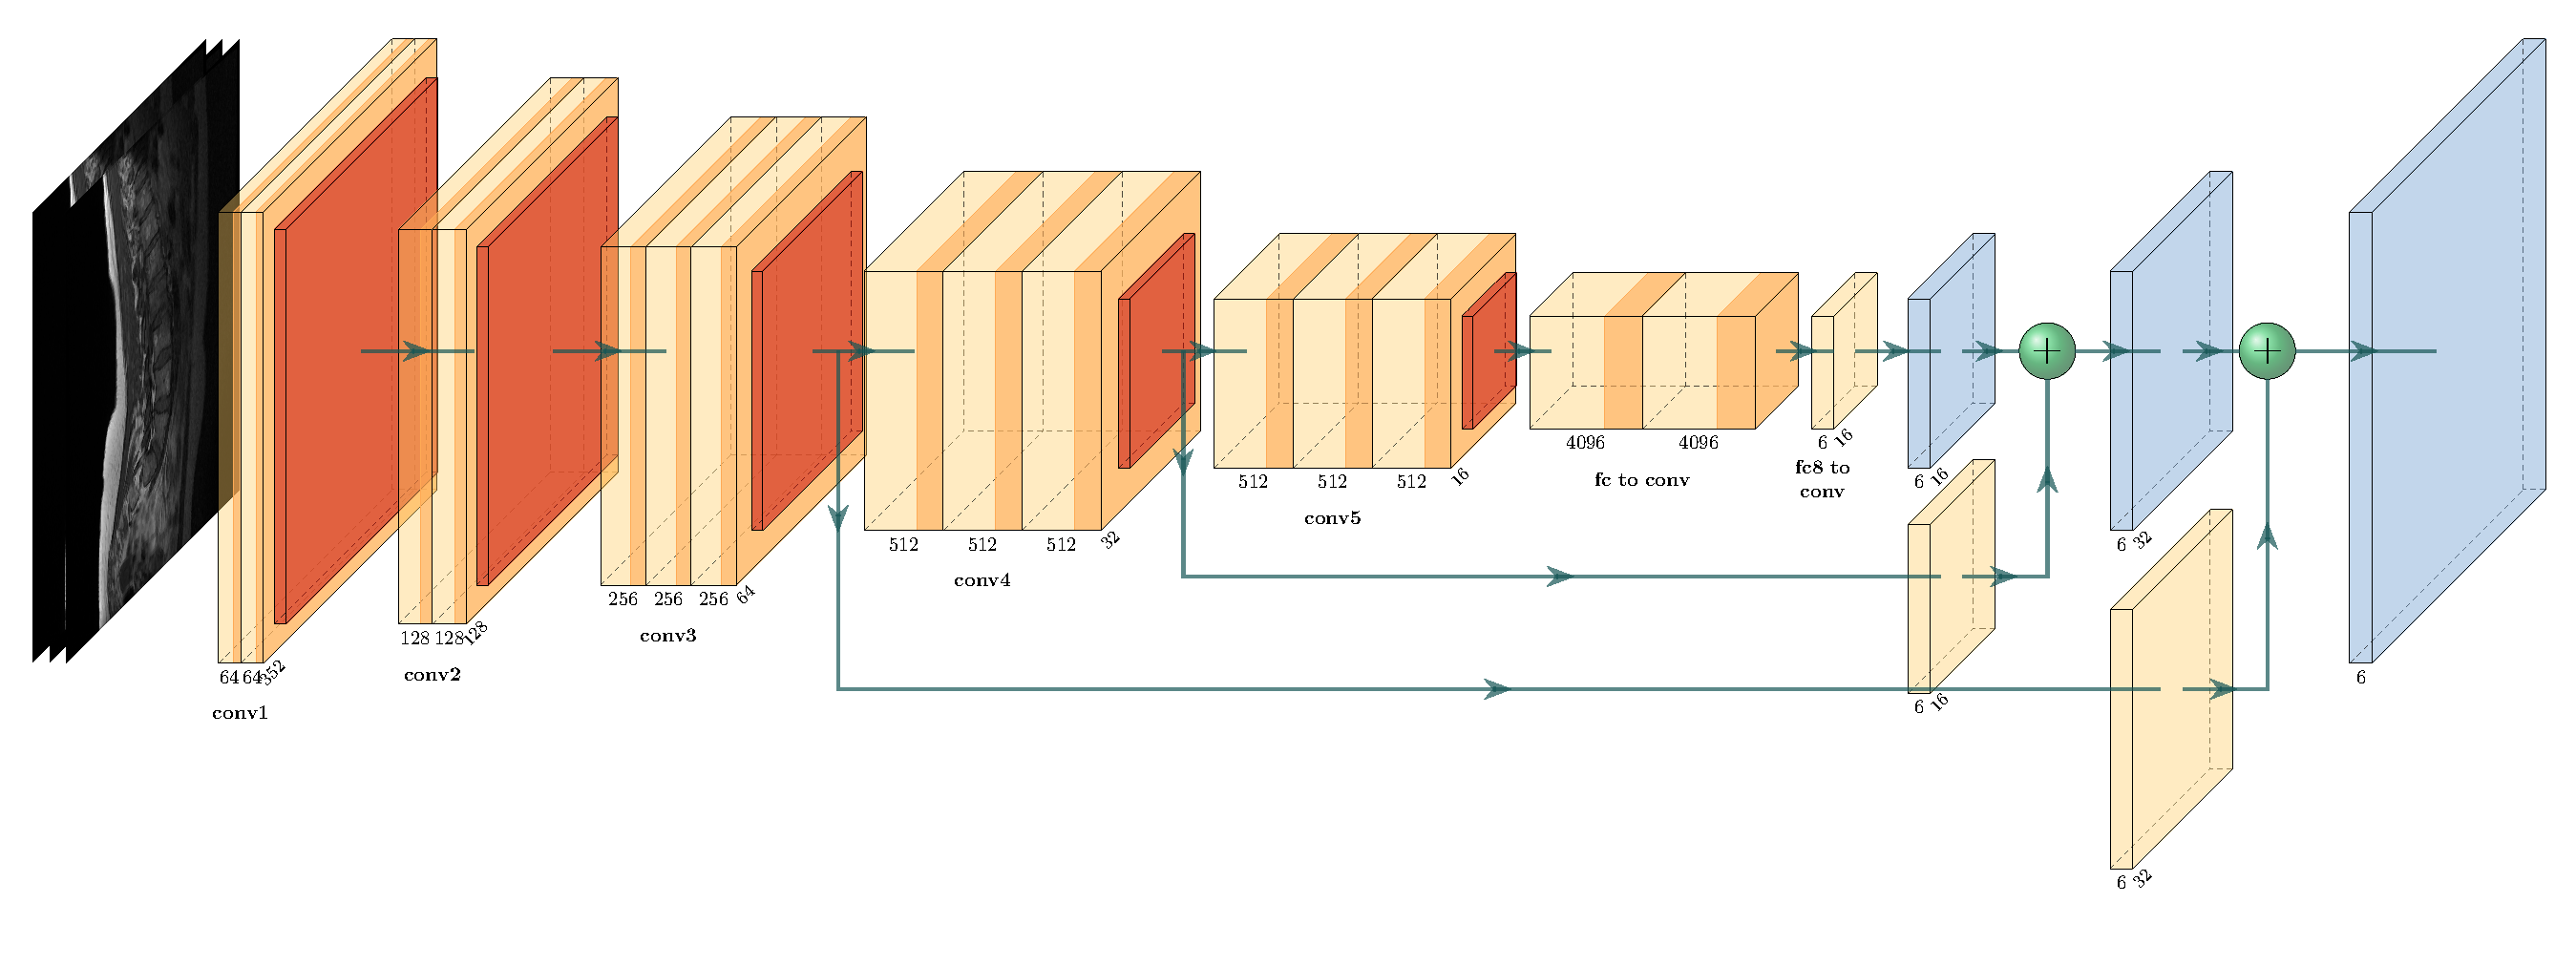
\includegraphics[width=.99\textwidth]{images/VGG16_FCN8.pdf}
    \end{minipage} 
    \vspace{2 mm}
    \begin{minipage}{.99\textwidth}
        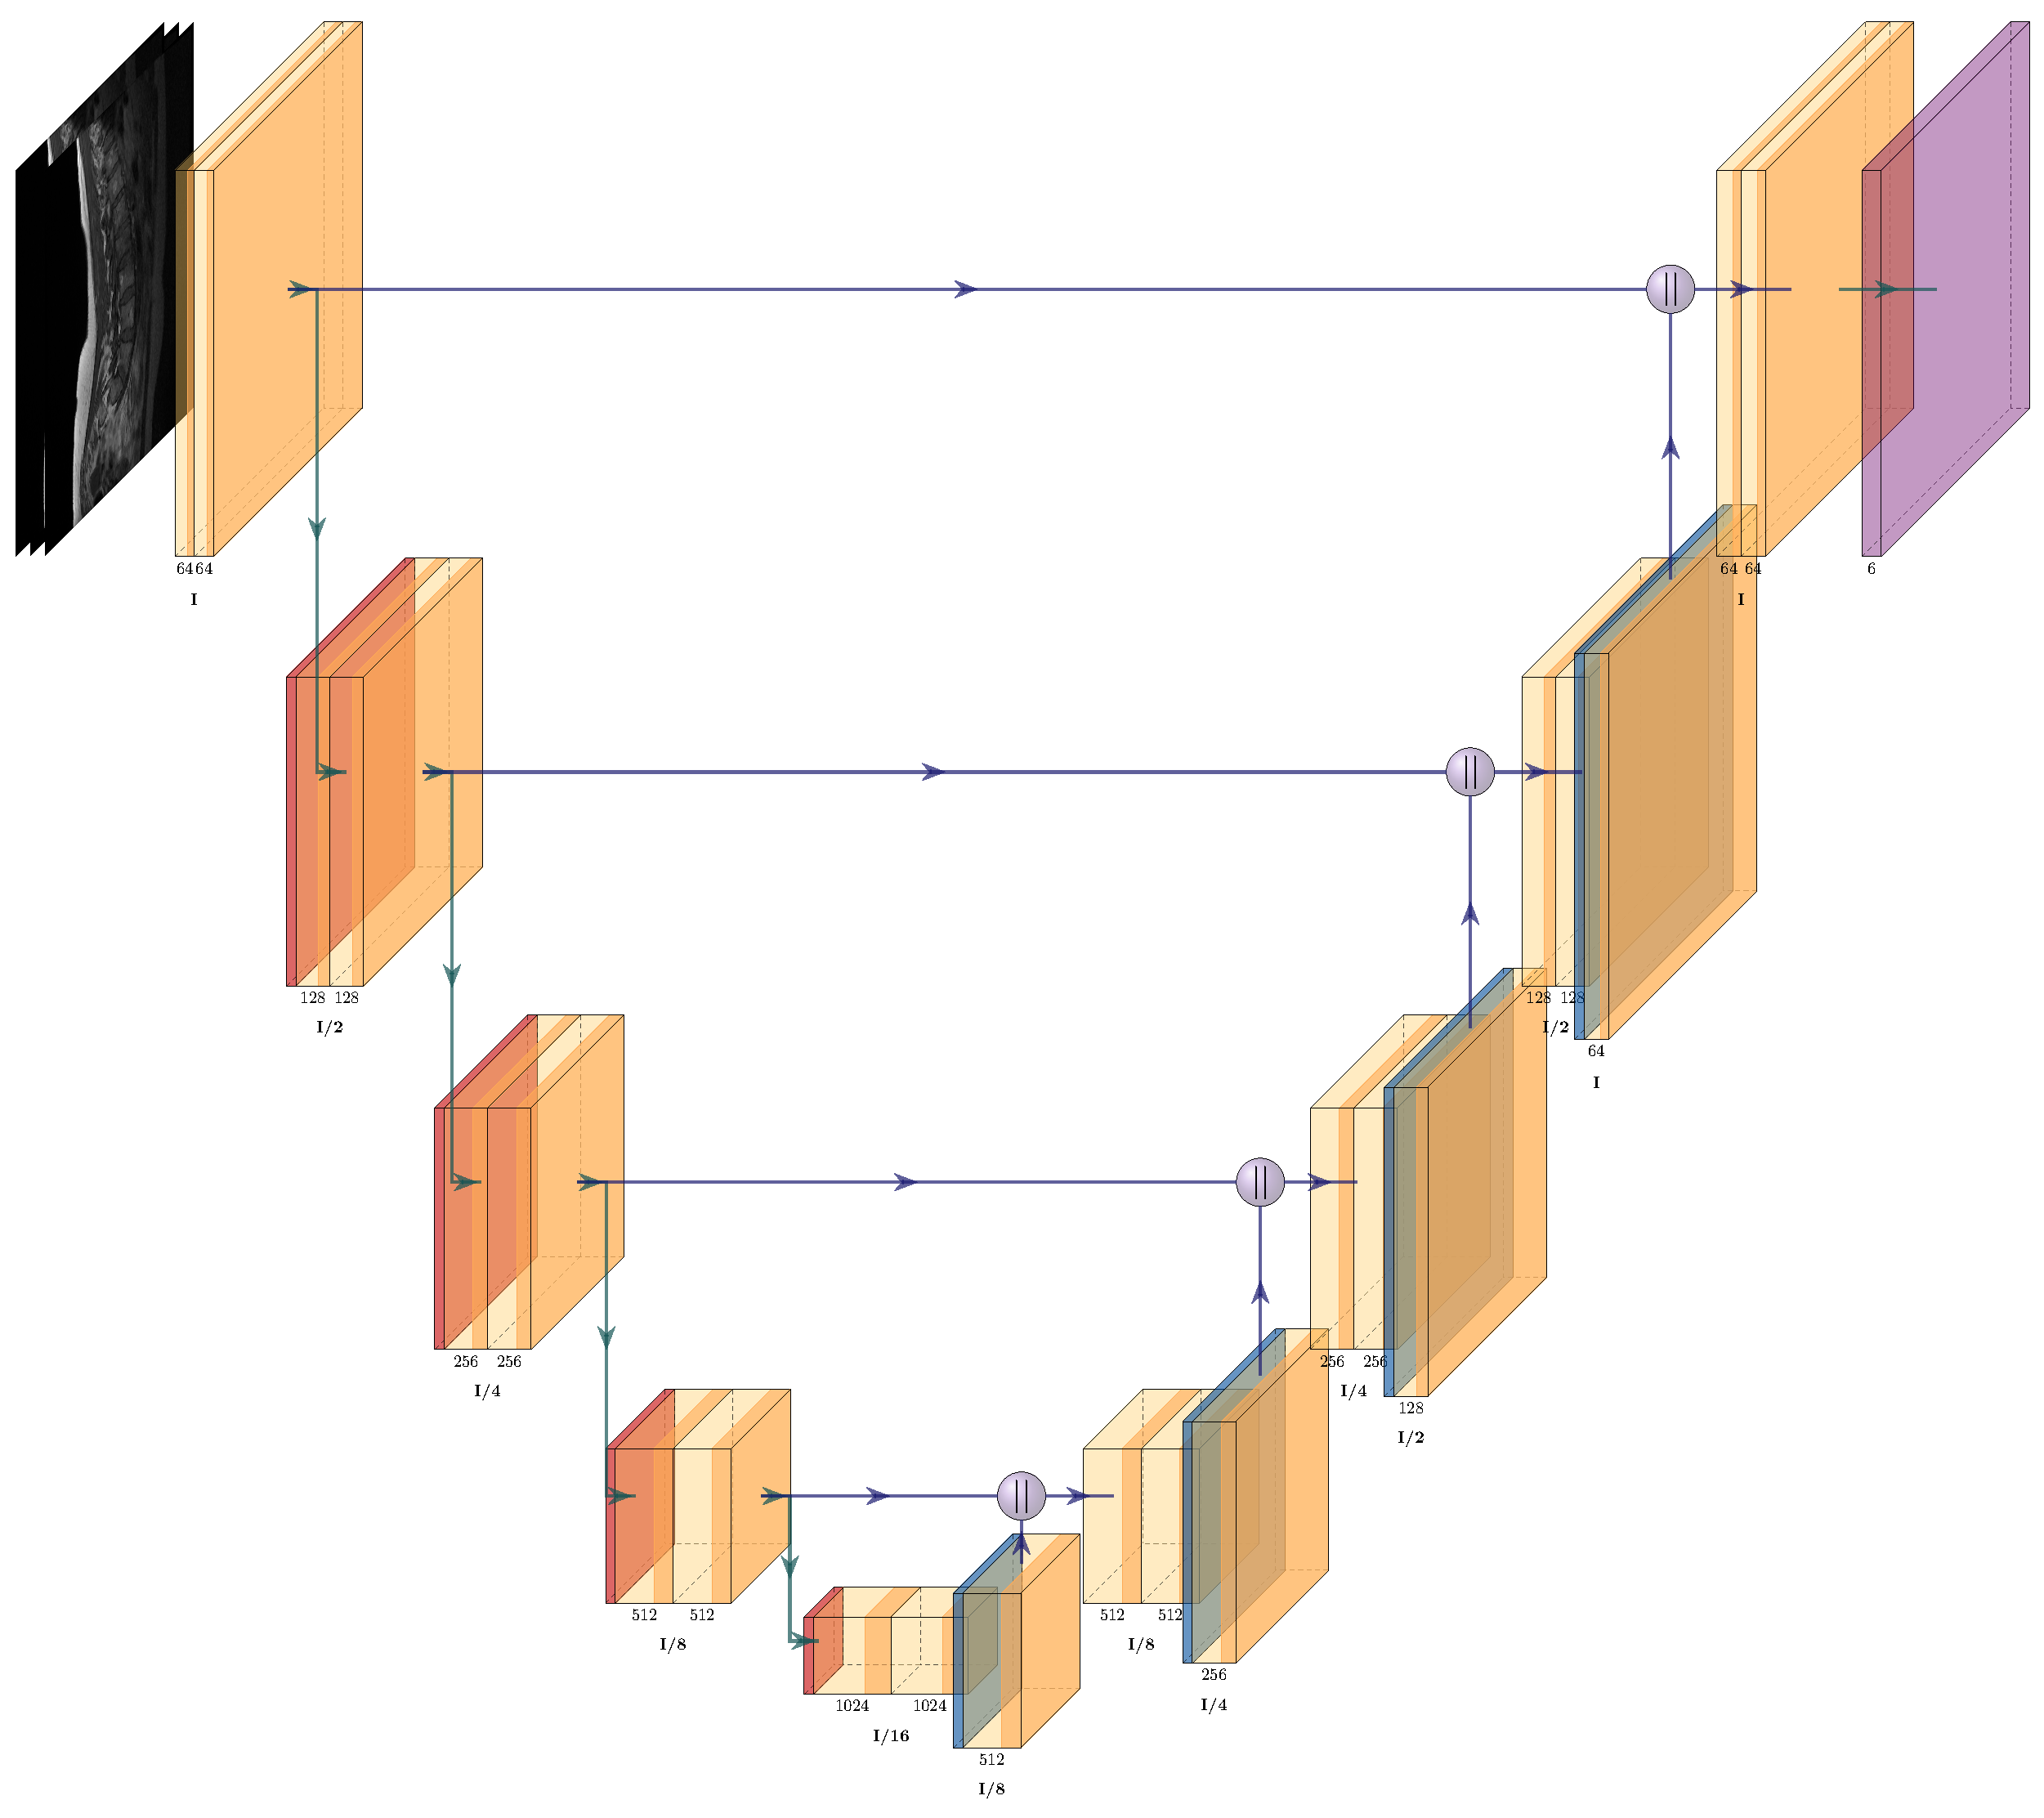
\includegraphics[width=.99\textwidth]{images/UNET.pdf}
    \end{minipage} 
     
    \caption{Illustrations of the tested network architectures.
    The first network is the VGG16-FCN8 network. \newline
    Then the U-Net architecture is illustrated. 
    \label{fig:vgg16}}
\end{SCfigure}
\begin{SCfigure}[][htb]
\begin{minipage}{.99\textwidth}
        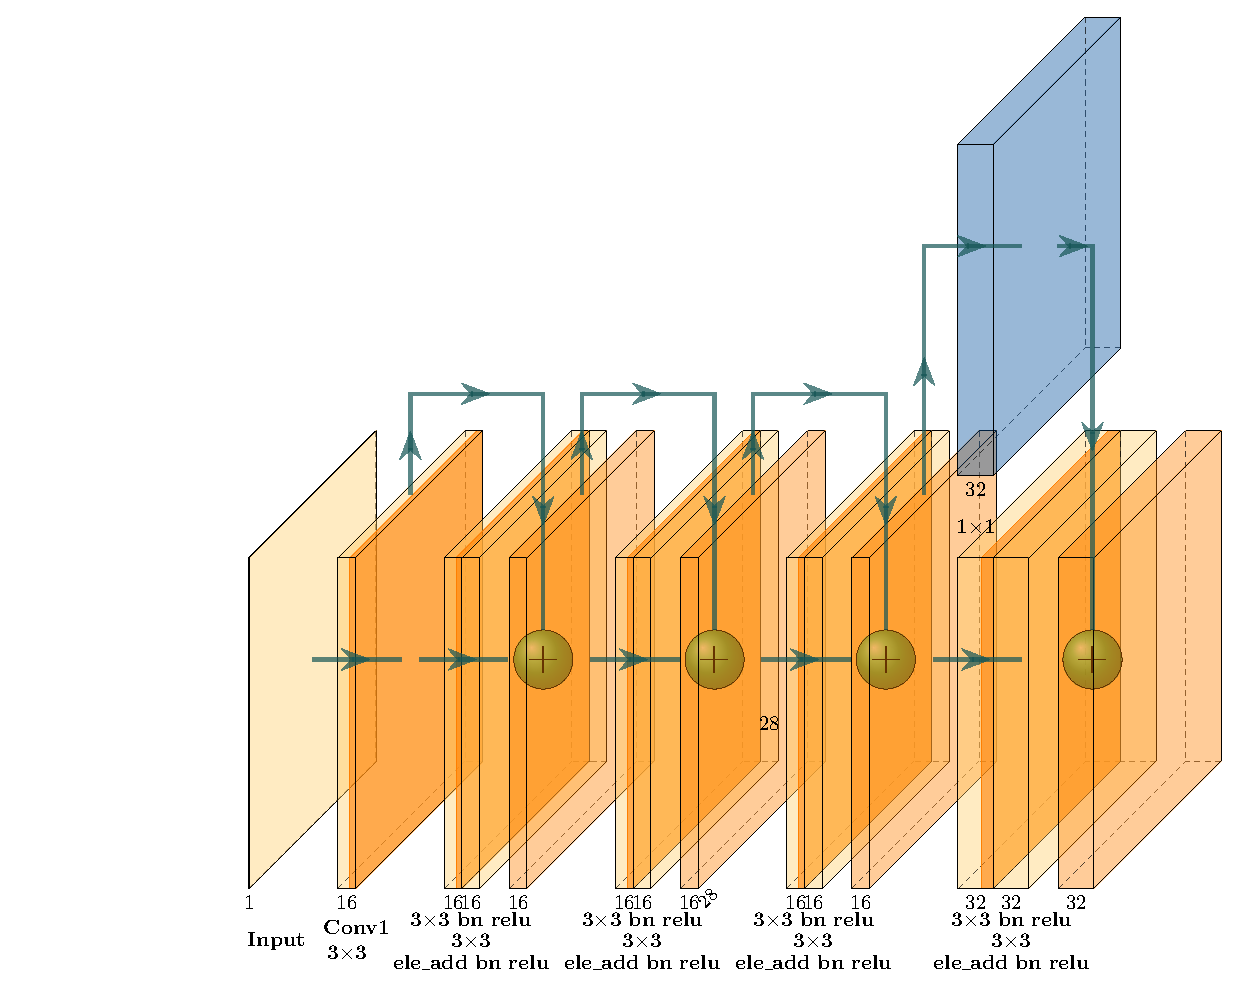
\includegraphics[width=.7\textwidth]{images/RESNET.pdf}
    \end{minipage}
    \caption{
One residual unit of the RESNET50 architecture.
    Due to the size of the RESNET50 network, only one \textit{residual block} is illustrated.
    }
\end{SCfigure}


\subsection{2D+ approach and \textit{context slices}\label{section:twoDplus}}

As discussed in section \ref{sec:network_types}, all used networks have a 3 channel\footnote{The networks were designed initially for \textit{RGB}-images with a red, a green and a blue channel.}, 
352$\times$352 pixel input. 
The input images for the network only have 1 channel component. 
The other two channels were used to pass \textit{context} information to the network in the form of the neighbouring slices of the slice under investigation.
This combines an essentially 2D approach with a third-dimensional element in the form of the extra information of the parallel slices. Thus, this is called the $2D+$ approach.

The hyperparameter to be set $k$ is the index offset for the context slices.
When evaluating slice with index $n$ the slices with indices $\left[n-k; n+k\right]$ are passed as context slices
\footnote{For the edge cases ($n<k$ or $n+k>$ image dimension) when these slices do not exist, slice $n$ is passed as context slice.}.

Several values for $k$ are tested. When $k=0$, no extra slices are taken. The same slice is just entered in all 3 network channels. When $k=1$, the indices directly next to the investigated slices are taken.
Due to the isotropic resampling (see section \ref{sec:resampling}), these slices are physically at a 1 mm distance from the centre slice. When $k=5$, the slices at $5 mm$ distance from the centre slice are used.

This stack of 3 slices is then passed through the network, as illustrated in figure \ref{fig:vgg16}.

\begin{SCfigure}[][htb]
    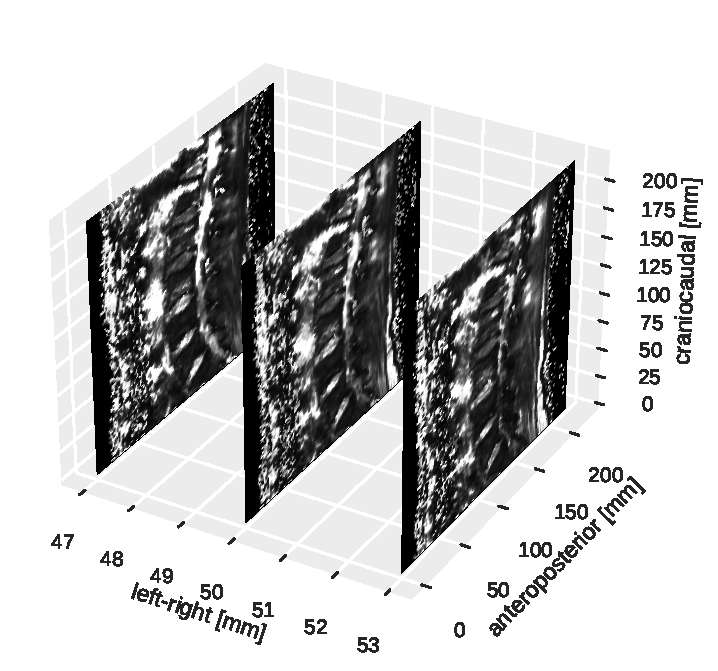
\includegraphics[width=.99\textwidth]{images/Context_slices.pdf}
    \caption{Illustration of the \textit{context slice} concept. Together with the image slice crop in the middle, the model input consists of the two slices at $k=3mm$ from the middle slice.}
\end{SCfigure}

\subsection{Annotation points\label{sec:annotationPoints}}
\par{
    An important hyperparameter is the number of annotation points per instance slice.
    This consists of two parameters: the background annotation points and the class annotation points.
    In this work, these are generated from the full masks provided in 4 of the 5 datasets.
    In every slice, annotation points are samples from the available masks in this slice.
}
\par{
    This project aims to investigate how the performance of a segmentation model trained on fully supervised data can be approximated with a model trained on weakly-supervised (point annotated) data.
    In the first place, this will be investigated by comparing models trained on the fully annotated data to models trained only with point labels generated based on the full masks.
    The generation of these point labels is automated. 
    The desired number of point labels is generated from the full segmentation ground by random selection of points from these masks.
    I did not investigate how closely point annotations generated in this way resemble point annotations generated by a human expert.
}
\begin{SCfigure}[][htb]
    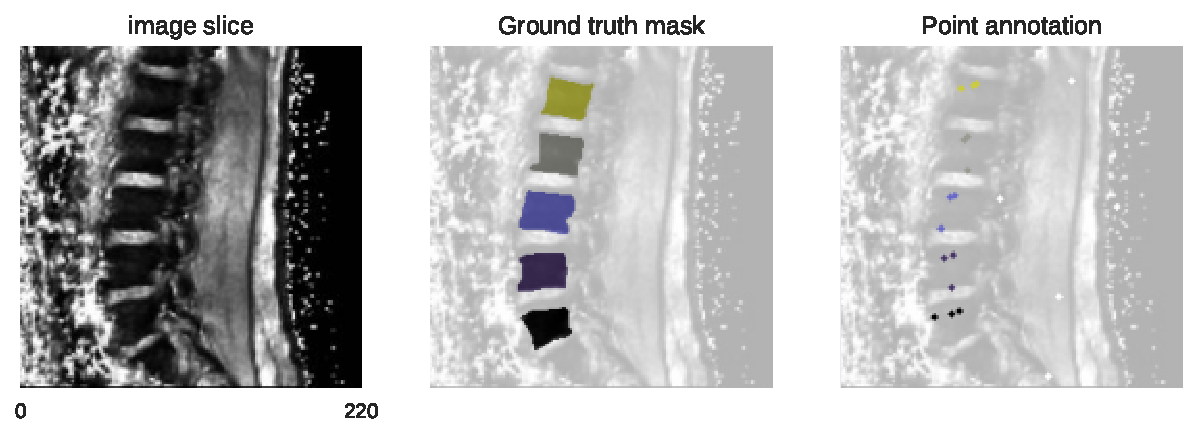
\includegraphics[width=.99\textwidth]{images/MyoSegmenTUM020_s21_points.pdf}
    \caption{This image illustrates how the \Gls{groundtruth} mask for MyoSegmenTUM image 020 (sagittal slice 21) is converted from a full annotation mask to a point annotation mask.
    \protect\newline\noindent Colour legend: \newline
\noindent\mycircle{colL1}  L1 %\newline 
\hspace{2mm}\mycircle{colL2}  L2 %\newline 
\hspace{2mm}\mycircle{colL3}  L3 %\newline 
\hspace{2mm}\mycircle{colL4}  L4 %\newline 
\hspace{2mm}\mycircle{colL5}  L5
    }
\end{SCfigure}
\par{
    In the first part of the research, the aim is to evaluate the difference between a model trained on a fully labelled set of images and a model trained on the same set of images for which only weak labels are provided.
    For this purpose, annotation points are generated for each slice.
    The individual models are thus trained with a fixed number of points per class instance in each slice,  approximating the situation where an expert annotates not one but three piles of slices, one for each dimension. The latter is not the final objective of this research.
    Based on the results obtained from this first step, three models are now trained based on a single set of annotation points, obtained from the annotation of slices along one dimension of the volume.
    Apart from the slices along the chosen dimension, the number of annotation points in the other two dimensions is not fixed.
}
%\FloatBarrier

\subsection{Model training strategy}

To optimize the model weights, the optimization scheme in algorithm \ref{alg:model_training} is executed.
The goal is to obtain model weights $\theta_b$ which show the best model performance, measured with metric $\mathcal{M}$ on the validation set $\mathcal{S}_{val}$.
This is done by evaluating the model with a pre-defined set of learning late reduction factors $\vec{f}_{LR}$ until the chosen metric $\mathcal{M}$ does not decrease anymore with decreasing training loss\footnote{
    This is tracked with the counter $T_\mathcal{M}$. Every time a training loss $\mathcal{L}_n$ is obtained lower than the best training loss $\mathcal{L}_b$ obtained up to that point, 
    the performance metric is compared to the best performance metric obtained up to that point. 
    If not improvement of the model performance metric can be observed $T_{\mathcal{M}, max}$ times in a row, the model training is halted, and the model weights are restored to $\theta_b$, the best performing set of weights.
    Evaluating more epochs would only result in overtraining the model to $\mathcal{S}_{train}$.
    \\[5pt]
    There is also a second counter: $T_\mathcal{L}$. If the optimizer is not able to decrease the model loss further with a given learning rate for a given number of epochs $T_{\mathcal{L}, max}$, the learning rate will be decreased with a factor defined in $\vec{f}_{LR}$.
    Since $\vec{f}_{LR}$ is finite, it is indeed possible that the optimization will be stopped because the model is still not capable of decreasing the loss at the last learning rate reduction.
}.


\begin{algorithm}[H]
    \SetAlgoLined
    \KwData{
        Train set $\mathcal{S}_{train}$ with weak annotations \;
        Validation set $\mathcal{S}_{val}$ with full annotations \;
        Test set $\mathcal{S}_{test}$ with full annotations \; 
    }
    \KwResult{
        Trained model weights $\theta_b$ \;
        Train, cross-validation and test metrics \;
        }
    \textbf{Algorithm:} \\
    $\mathcal{M}_b \leftarrow -\infty $ (best metric)\;
    $\mathcal{L}_b \leftarrow \infty $ (best loss)\;
    $LR \leftarrow 10^{-4}$ \;
    $\vec{f}_{LR} \leftarrow \left[ 1, 10, 10, 50 \right] $ \;
    $T_{\mathcal{M}} \leftarrow$ 0 \;
    $T_{\mathcal{M}, max} \leftarrow $ 10 \;

    \For{$fact_{LR} \in \vec{f}_{LR}$}{
        $LR \leftarrow LR / fact_{LR}$ \;
        $T_{\mathcal{L}} \leftarrow $ 0 \;
   \While{$T_{\mathcal{L}} < T_{\mathcal{L}, max} $}{
       $\mathcal{L}_n \leftarrow $ train epoch( $\mathcal{S}_{train}$ ) \;
       $\mathcal{M}_n \leftarrow $ evaluate($\mathcal{S}_{val}$) \;
       \eIf{$\mathcal{L}_n < \mathcal{L}_b$}{
            $T_{\mathcal{L}} \leftarrow 0$ \;
            $\mathcal{L}_b \leftarrow \mathcal{L}_n$ \;
             \eIf{$\mathcal{M}_n > \mathcal{M}_b$}{
                $T_\mathcal{M} \leftarrow 0$ \;
                $\mathcal{M}_b \leftarrow \mathcal{M}_n$ \;
                $\theta_b \leftarrow $ current model weights \; 
             }{
                $T_{\mathcal{M}} \leftarrow T_{\mathcal{M}} + 1$ \;
             }
            }{
                $T_{\mathcal{L}} \leftarrow T_{\mathcal{L}} + 1$ \;
            }
    }
   }
   set model weights to $\theta_b$ \;
   evaluate all metrics on $\mathcal{S}_{train}$, $\mathcal{S}_{train}$ \& $\mathcal{S}_{test}$ \;
    
    \caption{Model optimization strategy\label{alg:model_training}. The metric $\mathcal{M}$ used in this algorithm is the inverse class weighted dice score, etailed in equation \ref{eq:weighted_dice} on page \pageref{eq:weighted_dice}.}
\end{algorithm}

\par{
    The used optimization algorithm is \textit{Adam}, or Adaptive Moment estimating.
    This is a widely used and performant optimizer that has proven to work well in practice.
    This optimizer is started with a learning rate of $10^{-4}$.
    The learning rate can be reduced several times during the optimization procedure.
    In algorithm \ref{alg:model_training}, the full optimization procedure is described.
}